\documentclass[a4paper, titlepage]{jsarticle}

\usepackage[dvipdfmx]{graphicx}
\usepackage[dvipdfmx]{hyperref}
\usepackage{pxjahyper}
\usepackage{amsmath}
\usepackage{mathtools}
\usepackage{listings}

\lstset{
  basicstyle={\ttfamily},
  identifierstyle={\small},
  commentstyle={\smallitshape},
  keywordstyle={\small\bfseries},
  ndkeywordstyle={\small},
  stringstyle={\small\ttfamily},
  frame={tb},
  breaklines=true,
  columns=[l]{fullflexible},
  numbers=left,
  xrightmargin=0zw,
  xleftmargin=3zw,
  numberstyle={\scriptsize},
  stepnumber=1,
  numbersep=1zw,
  lineskip=-0.5ex
}

\title{知能システムⅡレポート4}
\author{三浦夢生}
\date{2021年1月3日}

\begin{document}
	\maketitle

	\section{目的}
	ディープラーニングに用いられる手法やライブラリ,モデルの構築や評価の方法を実際にプログラムを動かすことを通して学ぶ.

	\section{前提知識}
	今回用いたライブラリについて簡単な解説を行う.
	
	\subsection{TensorFlow}
	Googleが提供するオープンソースの機械学習ライブラリだが,機械学習に限らずテンソル計算も行える.
	また,大量の画像などのデータセットも提供している.
	クラウドやブラウザ,モバイルやIoTデバイス上などでも構築でき,様々なサービスを支える技術となっている.

	データフローグラフを用いることで複雑なネットワークを記述でき,また柔軟にネットワークを構築できる.
	後述するKerasも含まれているが,データフローを考慮して構築する必要があるため,初心者には少々難易度が高い.

	\subsection{Keras}
	Pythonで書かれた高水準の機械学習ライブラリのこと.内部的にはTensorFlowで計算を行っており,Kerasは多少の柔軟性を引き換えに機械学習の難易度を下げている.
	TensorFlowと同様にデータセットの提供もしている.

	数行のコードだけでモデルの構築,トレーニング,評価が可能であり,機械学習の入門ハードルが大幅に下げられたとも言われている.

	\subsection{CIFAR-10}
	Kerasから呼び出して利用ができるデータセットで,学習に利用できる.

	6万枚もの乗り物や動物のラベル付きカラー画像で,学習やベンチマークに利用されている.

	\section{方法}
	Colab上で付録に示すソースコードを実行し,結果を得,考察する.

	\section{結果}
	より画像の学習を得意とするCNNのほうが高い正解率を出せるモデルの作成に成功した.
	しかし,ネットワークの複雑さからかCNNのほうが時間がかかった.

	以下,正解率及びロスのグラフを示す.

	\subsection{MLPによる学習の結果}
	\begin{figure}[ht]
		\begin{tabular}{c}
			\begin{minipage}{0.5\hsize}
				\centering
				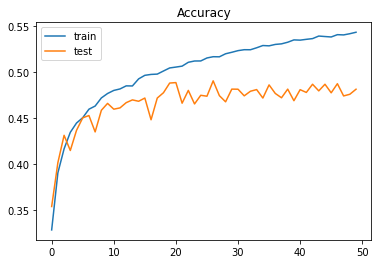
\includegraphics[keepaspectratio, scale=0.45]{result1-1.png}
			\end{minipage}
			\begin{minipage}{0.5\hsize}
				\centering
				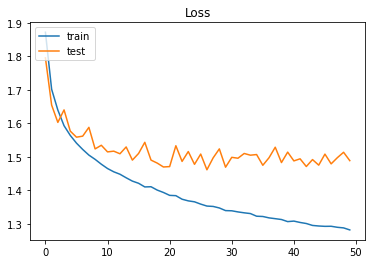
\includegraphics[keepaspectratio, scale=0.45]{result1-2.png}
			\end{minipage}
		\end{tabular}
	\end{figure}

	\subsection{CNNによる学習の結果}
	\begin{figure}[ht]
		\begin{tabular}{c}
			\begin{minipage}{0.5\hsize}
				\centering
				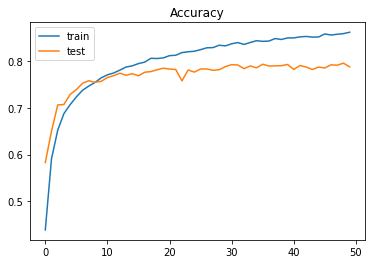
\includegraphics[keepaspectratio, scale=0.45]{result2-1.png}
			\end{minipage}
			\begin{minipage}{0.5\hsize}
				\centering
				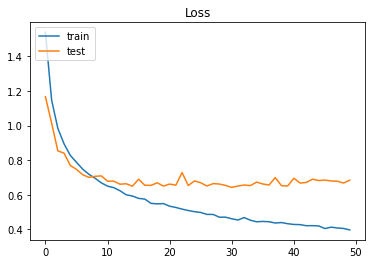
\includegraphics[keepaspectratio, scale=0.45]{result2-2.png}
			\end{minipage}
		\end{tabular}
	\end{figure}

	\section{付録}
	今回用いたソースコードを以下に示す.

	\subsection{MLPによる学習}
	MLP(Multi Layer Perceptron)とは,入力層・中間層・出力層の少なくとも3層からなる順伝播型ニューラルネットワークである.
	
	学習にはバックプロパゲーションを用いる.今回のソースコードではAdamを最適化アルゴリズムとし,多クラス交差エントロピーを損失関数としている.
	Adamとは慣性項を追加するモーメンタム法と学習率を調整するRMSPropを組み合わせた,現在デファクトスタンダードとなっている最適化アルゴリズムである.
	また,多クラス交差エントロピー(Categorical Cross Entropy)とはモデルの出力のlog値と正解をかけたものの総和を損失とする手法である.損失関数の値が大きいときに学習幅が大きいために学習スピードが速い.

	\begin{lstlisting}
import matplotlib.pyplot as plt
import keras
from keras.datasets import cifar10
from keras.models import Sequential
from keras.layers import Dense, Dropout

num_classes = 10
im_rows = 32
im_cols = 32
im_size = im_rows * im_cols * 3

(X_train, y_train), (X_test, y_test) = cifar10.load_data()

X_train = X_train.reshape(-1, im_size).astype('float32') / 255
X_test = X_test.reshape(-1, im_size).astype('float32') / 255

y_train = keras.utils.to_categorical(y_train, num_classes)
y_test = keras.utils.to_categorical(y_test, num_classes)

model = Sequential()
model.add(Dense(512, activation='relu', input_shape=(im_size,)))
model.add(Dense(num_classes, activation='softmax'))

model.compile(
    loss='categorical_crossentropy',
    optimizer='adam',
    metrics=['accuracy']
)

hist = model.fit(X_train, y_train, batch_size=32, epochs=50, verbose=1, validation_data=(X_test, y_test))

score = model.evaluate(X_test, y_test, verbose=1)
print('seikai =', score[1], 'loss = ', score[0])

model.save('./gdrive/My Drive/Colab Notebooks/cifar10-mlp.h5')

plt.plot(hist.history['accuracy'])
plt.plot(hist.history['val_accuracy'])
plt.title('Accuracy')
plt.legend(['train', 'test'], loc='upper left')
plt.show()
plt.plot(hist.history['loss'])
plt.plot(hist.history['val_loss'])
plt.title('Loss')
plt.legend(['train', 'test'], loc='upper left')
plt.show()	
	\end{lstlisting}

	\subsection{CNNによる学習}
	CNN(Convolutional Neural Network)とは,通常のニューラルネットワークに「畳み込み」や「プーリング」といった処理を追加したものであり,画像の深層学習においてメジャーな手法である.

	畳み込みとは,カーネル(フィルターとも言う)という格子状の数値データと,それと同サイズの元画像の一部の数値データに関して各要素の積の和を計算することで一つの数値を得(これをテンソルという),これを繰り返すことで特徴マップを作成することである.
	またプーリングとは,ウィンドウと呼ばれるサイズで画像の一部にフォーカスを当てて,数値を作り出すことで,ウィンドウのうち最大値を選ぶ手法を最大値プーリングといい,ウィンドウ内の平均値をとる手法を平均値プーリングという.

	また以下のモデルは画像認識コンテストで優秀な成績を収めたチームが作成したモデルに似ていることからVGG likeと呼ばれている.

	\begin{lstlisting}
import matplotlib.pyplot as plt
import keras
from keras.datasets import cifar10
from keras.models import Sequential
from keras.layers import Dense, Dropout, Activation, Flatten
from keras.layers import Conv2D, MaxPooling2D

num_classes = 10
im_rows = 32
im_cols = 32
in_shape = (im_rows, im_cols, 3)

(X_train, y_train), (X_test, y_test) = cifar10.load_data()

X_train = X_train.astype('float32') / 255
X_test = X_test.astype('float32') / 255

y_train = keras.utils.to_categorical(y_train, num_classes)
y_test = keras.utils.to_categorical(y_test, num_classes)

model = Sequential()
model.add(Conv2D(32, (3, 3), padding='same', input_shape=in_shape))
model.add(Activation('relu'))
model.add(Conv2D(32, (3, 3)))
model.add(Activation('relu'))
model.add(MaxPooling2D(pool_size=(2, 2)))
model.add(Dropout(0.25))

model.add(Conv2D(64, (3, 3), padding='same'))
model.add(Activation('relu'))
model.add(Conv2D(64, (3, 3)))
model.add(Activation('relu'))
model.add(MaxPooling2D(pool_size=(2, 2)))
model.add(Dropout(0.25))

model.add(Flatten())
model.add(Dense(512))
model.add(Activation('relu'))
model.add(Dropout(0.5))
model.add(Dense(num_classes))
model.add(Activation('softmax'))

model.compile(
    loss='categorical_crossentropy',
    optimizer='adam',
    metrics=['accuracy']
)

hist = model.fit(X_train, y_train, batch_size=32, epochs=50, verbose=1, validation_data=(X_test, y_test))

score = model.evaluate(X_test, y_test, verbose=1)
print('seikai =', score[1], 'loss = ', score[0])

model.save('./gdrive/My Drive/Colab Notebooks/cifar10-cnn.h5')

plt.plot(hist.history['accuracy'])
plt.plot(hist.history['val_accuracy'])
plt.title('Accuracy')
plt.legend(['train', 'test'], loc='upper left')
plt.show()
plt.plot(hist.history['loss'])
plt.plot(hist.history['val_loss'])
plt.title('Loss')
plt.legend(['train', 'test'], loc='upper left')
plt.show()
	\end{lstlisting}
\end{document}
